\documentclass{beamer}


\usetheme{Ilmenau}

\title{Matrix Project}

\subtitle{EE1390}

\author{Gaurav Gijare - EP17BTECH11007 \linebreak Aditya Patel - EP17BTECH11002}


\institute[Indian Institute of Technology, Hyderabad] % (optional, but mostly needed)
{
  \inst{}%
  Indian Institute of Technology, Hyderabad
}

\date{February 14, 2019}

\AtBeginSubsection[]
{
  \begin{frame}<beamer>{Outline}
    \tableofcontents[currentsection, currentsubsection]
  \end{frame}
}

% Let's get started
\begin{document}

\begin{frame}
  \titlepage
\end{frame}

\begin{frame}{Outline}
  \tableofcontents
\end{frame}

\section{Matrix Analysis}

\subsection{Geometry Question}

\begin{frame}{Geometric Question}{Question 1}
  {
  Q1. Tangent and normal are drawn at \(\textbf{P} = \begin{pmatrix}{-16\\16}\end{pmatrix}\) on the parabola \(\textbf{x}^T\begin{pmatrix}{0 & 0\\0 & 1}\end{pmatrix}\textbf{x} + \begin{pmatrix}{16 & 0}\end{pmatrix}\textbf{x} = 0\) which intersect the axis of the parabola at \textbf{A} and \textbf{B} respectively. If \textbf{C} is the centre of the circle through the points \textbf{P}, \textbf{A} and \textbf{B}, find \textbf{tan CPB}.
  }
\end{frame}

\subsection{Matrix transformation of the question}

\begin{frame}{Matrix transformation of the question}{}
  {
    The general equation of a conic in matrix form is: 
   \[ \textbf{x}^T\textbf{V}\ \textbf{x} + 2 \textbf{U}^T\ \textbf{x} + \textbf{F} = 0\]
   Comparing with the given equation of parabola:
   \[ \textbf{x}^T\begin{pmatrix}{0 & 0\\0 & 1}\end{pmatrix}\textbf{x} + \begin{pmatrix}{16 & 0}\end{pmatrix}\textbf{x} = 0 \]
  }
\end{frame}

\begin{frame}{Matrix transformation of the question}{}
    {
        We get,\linebreak
        \[ \textbf{V} = \begin{pmatrix}{0 & 0\\0 & 1}\end{pmatrix} \qquad
        \textbf{U} = \begin{pmatrix}{8 \\ 0}\end{pmatrix} \] \linebreak
        \[\textbf{F} = \begin{bmatrix}{0}\end{bmatrix} \]
    }
\end{frame}

\subsection{Solution in form of matrix}
\begin{frame}{Solution using matrices}{}
  {
    The equation of a tangent to the parabola at point \textbf{P} is: 
   \[ \begin{pmatrix}{\textbf{P}^T & 1}\end{pmatrix} \begin{pmatrix}{\textbf{V} & \textbf{U} \\ \textbf{U}^T & \textbf{F}}\end{pmatrix} \begin{pmatrix}{\textbf{x} \\ 1}\end{pmatrix} = 0 \]
   It can also be expressed as:
   \[ \begin{pmatrix}{\textbf{P}^T\textbf{V} + \textbf{U}^T}\end{pmatrix}\textbf{x} + \textbf{P}^T\textbf{U} + \textbf{F} = 0 \]
   Therefore, the equation of tangent becomes:
    \[ \begin{bmatrix}{ \begin{pmatrix}-16 & 16\end{pmatrix} \begin{pmatrix}0 & 0 \\ 0 & 1\end{pmatrix} + \begin{pmatrix}8 & 0\end{pmatrix}}\end{bmatrix}\textbf{x} + \begin{pmatrix}-16 & 16\end{pmatrix} \begin{pmatrix}8 \\ 0\end{pmatrix} = 0 \]
  }
\end{frame}

\begin{frame}{Solution using matrices}{}
  {
    Comparing with the equation of line, the normal vector of tangent will be: 
   \[ \textbf{n}^T = \begin{bmatrix}{ \begin{pmatrix}-16 & 16\end{pmatrix} \begin{pmatrix}0 & 0 \\ 0 & 1\end{pmatrix} + \begin{pmatrix}8 & 0\end{pmatrix}}\end{bmatrix} \implies \textbf{n} = \begin{pmatrix}8 & 16\end{pmatrix} \]
   Therefore, the direction vector for the tangent will be
   \[ \textbf{m}_t_a_n_g_e_n_t =  \begin{pmatrix}{0 & -1 \\ 1 & 0 }\end{pmatrix} \begin{pmatrix}{8 \\ 16 }\end{pmatrix} = \begin{pmatrix}{-16 \\ 8 }\end{pmatrix} \]
   Therefore, the equation of normal will be:
    \[ \textbf{X} = \begin{pmatrix}-16 \\ 16\end{pmatrix} + \lambda \begin{pmatrix}{8 \\ 16 }\end{pmatrix} \]
  }
\end{frame}

\begin{frame}{Solution using matrices}{}
  {
   Now, we have equation of tangent, normal as well as parabola. Lets visualize it:
   \begin{center}
       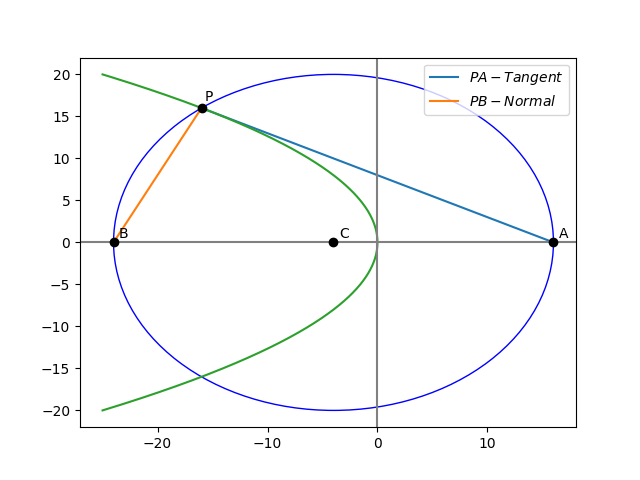
\includegraphics[width=6cm,height=6cm,keepaspectratio]{Figure_2.jpg}
   \end{center}
  }
\end{frame}

\begin{frame}{Solution using matrices}{}
  {
   Now, we have to draw a circle which passes through \textbf{B}, \textbf{P} and \textbf{A}:
   \begin{itemize}
   \item
        As normal and tangent at \textbf{P} are perpendicular to each other, seg \textbf{AB} will be the diameter of the circle with centre \textbf{C}.   \pause
   \item 
        The x-intercepts \quad \textbf{A} = \(\begin{pmatrix} 16 \\ 0\end{pmatrix}\) \qquad \textbf{B} = \(\begin{pmatrix} -24 \\ 0\end{pmatrix}\)  \pause
   \item
         Centre of circle = mid-point of \textbf{A} and \textbf{B} \linebreak \implies \textbf{C} = \(\begin{pmatrix} -4 \\ 0\end{pmatrix}\) \pause
   \item 
        Radius of the circle = distance between points \textbf{C} and \textbf{A} \linebreak \implies \textbf{R} = \(20\)
   \end{itemize}
  }
\end{frame}

\begin{frame}{Solution using matrices}{}
  {
   We have to find Tan \angle \textbf{CPB}:
   \begin{center}
       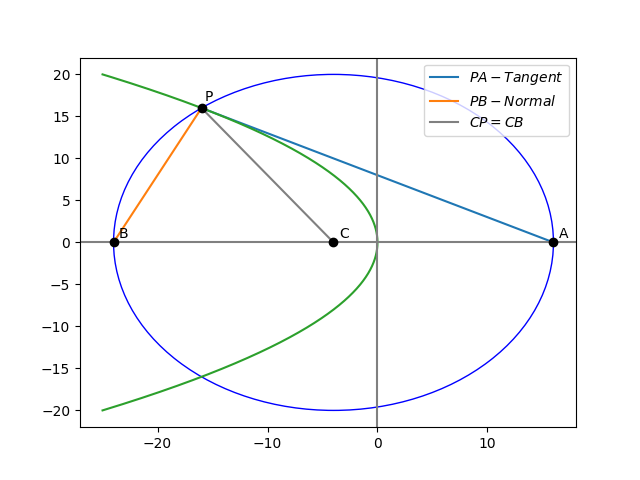
\includegraphics[width=9cm,height=9cm,keepaspectratio]{Figure_3.png}
   \end{center}
  }
\end{frame}

\begin{frame}{Solution using matrices}{}
  {
   \begin{itemize}
   \item 
        \textbf{CB} = \textbf{CP} = \textbf{CA} = \textbf{R} \pause
   \item 
        \(\angle \textbf{CPB} = \angle \textbf{CBP} \) \implies \(Tan\ \angle \textbf{CPB} = Tan\ \angle \textbf{CBP} \) \pause
   \item
        But \(Tan\ \angle \textbf{CBP}\) = slope of normal \textbf{BP}  \pause
   \item
        \therfore \( Tan\ \angle \textbf{CPB} = \dfrac{16}{8} = 2 \)   
   \end{itemize}
  }
\end{frame}

\subsection{Solution Figure}

\begin{frame}{Solution Figure}{}
  {
   \begin{center}
       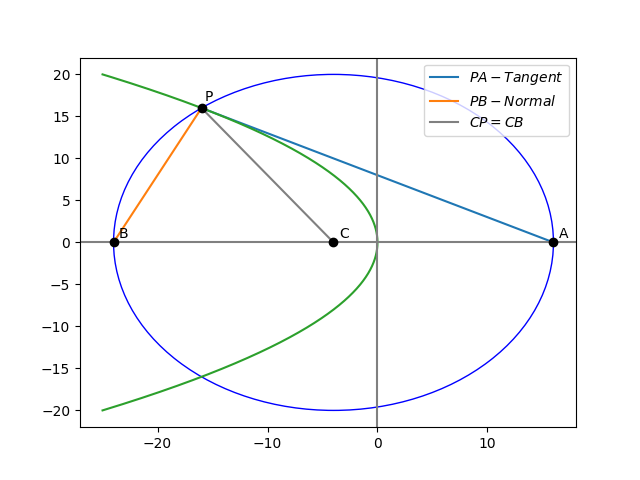
\includegraphics[width=7.8cm,height=7.8cm,keepaspectratio]{Figure_3.png}
   \end{center}
  }
\end{frame}


\end{document}


